% This LaTeX was auto-generated from MATLAB code.
% To make changes, update the MATLAB code and export to LaTeX again.

\documentclass{article}

\usepackage[utf8]{inputenc}
\usepackage[T1]{fontenc}
\usepackage{lmodern}
\usepackage{graphicx}
\usepackage{color}
\usepackage{hyperref}
\usepackage{amsmath}
\usepackage{amsfonts}
\usepackage{epstopdf}
\usepackage[table]{xcolor}
\usepackage{matlab}

\sloppy
\epstopdfsetup{outdir=./}
\graphicspath{ {./actividad1_2_images/} }

\begin{document}

\matlabtitle{Actividad Práctica N°1. Representación de sistemas y control PID.}

\matlabheading{Caso de estudio 2. Sistema de tres variables de estado.}

\matlabheadingtwo{Consigna}

\begin{par}
\begin{flushleft}
Dadas las ecuaciones del motor de corriente continua con torque de carga $T_L$ no nulo, con los parámetros:
\end{flushleft}
\end{par}

\begin{itemize}
\setlength{\itemsep}{-1ex}
   \item{\begin{flushleft} $\displaystyle L_{\textrm{AA}} =366\;{10}^{-6}$ \end{flushleft}}
   \item{\begin{flushleft} $\displaystyle J=5\;{10}^{-9}$ \end{flushleft}}
   \item{\begin{flushleft} $\displaystyle R_A =55\ldotp 6$ \end{flushleft}}
   \item{\begin{flushleft} $\displaystyle B_m =0$ \end{flushleft}}
   \item{\begin{flushleft} $\displaystyle K_i =6\ldotp 49\;{10}^{-3}$ \end{flushleft}}
   \item{\begin{flushleft} $\displaystyle K_m =6\ldotp 53\;{10}^{-3}$ \end{flushleft}}
\end{itemize}

\begin{par}
\begin{flushleft}
Modelado por las siguientes ecuaciones diferenciales:
\end{flushleft}
\end{par}

\begin{itemize}
\setlength{\itemsep}{-1ex}
   \item{\begin{flushleft} $\displaystyle \frac{{\textrm{di}}_a \;}{\textrm{dt}}=\frac{-R_A }{\;L_{\textrm{AA}} }*i_a -\frac{\;K_m }{\;L_{\textrm{AA}} }\omega_r +\frac{1\;}{L_{\textrm{AA}} }v_a$ \end{flushleft}}
   \item{\begin{flushleft} $\displaystyle \frac{d\omega_r }{\textrm{dt}}=\frac{K_i \;}{J}i_a -\frac{B_m \;}{J}\omega {\;}_r -\frac{1\;}{J}T_L$ \end{flushleft}}
   \item{\begin{flushleft} $\displaystyle \frac{d\Theta_t }{\textrm{dt}}=\omega_r$ \end{flushleft}}
\end{itemize}

\begin{par}
\begin{flushleft}
Implementar un algoritmo de simulación para inferir el comportamiento de las variables interés  mediante integración Euler con $\Delta t={10}^{-7}$segundos para:
\end{flushleft}
\end{par}

\begin{enumerate}
\setlength{\itemsep}{-1ex}
   \item{\begin{flushleft} Obtener el torque máximo que puede soportar el motor modelado mediante las ecuaciones diferenciales anteriores cuando se lo alimenta con $12V$, graficando para $5$ segundos de tiempo la velocidad angular y la corriente $i_a$. \end{flushleft}}
   \item{\begin{flushleft} Mostrar simulaciones de 5 segundos que permitan observar la corriente $i_a$ en todo momento y establecer su valor máximo como para dimensionar dispositivos electrónicos. \end{flushleft}}
   \item{\begin{flushleft} A partir de las curvas de mediciones de las variables graficadas, se requiere obtener el modelo del sistema considerando como entrada un escalón de $12V$, como salida a la velocidad angular, y a partir de $0\ldotp 1$ segundo se aplica un $T_L$ aproximado de $7\ldotp 5\;{10}^{-2} \;\textrm{Nm}$. En el archivo Curvas\_Medidas\_Motor.xls están las mediciones, en la primer hoja los valores y en la segunda los nombres. Se requiere obtener el modelo dinámico, para establecer las constantes de la corriente. \end{flushleft}}
   \item{\begin{flushleft} Implementar un PID en tiempo discreto para que el ángulo del motor permanezca en una referencia de $1\;\textrm{rad}$. (Tip: a partir de $K_P =0\ldotp 1;K_i =0\ldotp 01;K_D =5$). \end{flushleft}}
\end{enumerate}

\begin{par}
\begin{flushleft}
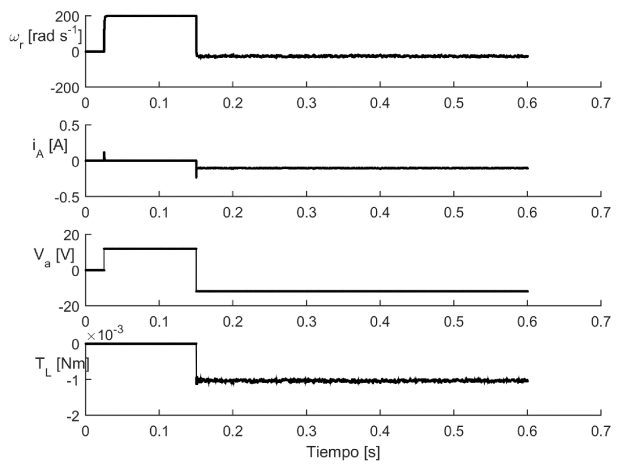
\includegraphics[width=\maxwidth{62.81986954340191em}]{image_0}
\end{flushleft}
\end{par}


\matlabheadingtwo{Resolución}

\begin{par}
\begin{flushleft}
En primera instancia se integran las dos primeras ecuaciones diferenciales haciendo uso del método de Integración de Euler, con el paso fijado en la consigna del ejercicio.
\end{flushleft}
\end{par}


\begin{par}
\begin{flushleft}
Primero se pasiva la entrada que responde al torque del motor, para integrar las ecuaciones de velocidad angular y corriente en función de la entrada de tensión. Se aplica el teorema de superposición.
\end{flushleft}
\end{par}

\begin{matlabcode}
T = 0.6;
deltaT = 1e-7;
Kmax = T/deltaT;
t = linspace(0,T,Kmax);

Laa = 366e-6;
J = 5e-9;
Ra = 55.6;
Bm = 0;
Ki = 6.49e-3;
Km = 6.53e-3;

Vin = 12;
iaP = 0;
wrP = 0;
Ia = zeros(1, Kmax);
Wr = zeros(1, Kmax);
u = linspace(0, 0, Kmax);
Ia(1) = 0;
Wr(1) = 0;
u(1) = Vin;

A = [-Ra/Laa -Km/Laa; Ki/J -Bm/J];
B = [1/Laa; 0];
C1 = [1 0];
C2 = [0 1];

Ial(1) = 0;
Wrl(1) = 0;
x = [Ia(1) Wr(1)]';
Xop = [0 0]';

ii = 0;
for i = 1:(Kmax-1)
    ii = ii+deltaT;
    if(ii>=0 && ii<0.025)
        Vin = 0;
    end
    if(ii>=0.025 && ii<0.15)
        Vin = 12;
    end
    if(ii>=0.15)
        Vin = -12;
    end
    u(i) = Vin;
    iaP = -(Ra/Laa)*Ia(i)-(Km/Laa)*Wr(i)+(1/Laa)*u(i);
    wrP = (Ki/J)*Ia(i)-(Bm/J)*Wr(i);
    xP = A*(x-Xop)+B*u(i);
    x = x+xP*deltaT;
    Y1 = C1*x;
    Y2 = C2*x;
    Ial(i+1) = x(1);
    Wrl(i+1) = x(2);
end
\end{matlabcode}

\begin{par}
\begin{flushleft}
A continuación, se grafican las dos salidas del sistema planteado para una entrada de tensión que inicia en $0V$, luego, al cabo de $0\ldotp 025\;\textrm{seg}$ comienza a valer $12V$, para luego, a los $0\ldotp 125\;\textrm{seg}$ cambiar su signo, pasando a valer $-12V$.
\end{flushleft}
\end{par}

\begin{matlabcode}
subplot(3,1,1);
plot(t,u,'LineWidth',3);
title('Tension de entrada v_a(t)');
xlabel('Tiempo [s]');
ylabel('Tension [V]');
grid;
subplot(3,1,2);
plot(t,Ial); 
title('Corriente de armadura i_a(t)');
xlabel('Tiempo [s]');
ylabel('Corriente [A]')
grid;
subplot(3,1,3);
plot(t,Wrl); 
title('Velocidad angular \omega_r(t)');
xlabel('Tiempo [s]');
ylabel('\omega_r [rad s^{-1}]')
grid;
\end{matlabcode}
\begin{center}
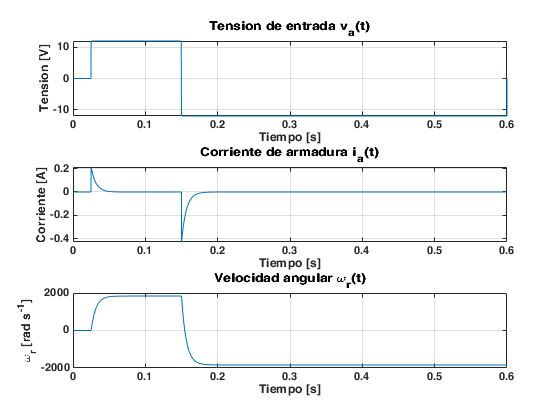
\includegraphics[width=\maxwidth{56.196688409433015em}]{figure_0.png}
\end{center}


\begin{par}
\begin{flushleft}
Las gráficas anteriores son para simplemente comparar resultados con las gráficas brindadas por la consigna. Ahora, para continuar con lo solicitado, se ingresará el escalón de tensión de $12\;V$ y se simulará el sistema durante $5\;\textrm{seg}$.
\end{flushleft}
\end{par}

\begin{matlabcode}
T = 5;
deltaT = 1e-7;
Kmax = 10000000;
t = linspace(0,T,Kmax);

Laa = 366e-6;
J = 5e-9;
Ra = 55.6;
Bm = 0;
Ki = 6.49e-3;
Km = 6.53e-3;

Vin = 12;
iaP = 0;
wrP = 0;
Ia = zeros(1, Kmax);
Wr = zeros(1, Kmax);
u = linspace(0, 0, Kmax);
Ia(1) = 0;
Wr(1) = 0;
u(1) = Vin;

A = [-Ra/Laa -Km/Laa; Ki/J -Bm/J];
B = [1/Laa; 0];
C1 = [1 0];
C2 = [0 1];

Ial(1) = 0;
Wrl(1) = 0;
x = [Ia(1) Wr(1)]';
Xop = [0 0]';

ii = 0;
for i = 1:(Kmax-1)
    ii = ii+deltaT;
    u(i) = Vin;
    iaP = -(Ra/Laa)*Ia(i)-(Km/Laa)*Wr(i)+(1/Laa)*u(i);
    wrP = (Ki/J)*Ia(i)-(Bm/J)*Wr(i);
    xP = A*(x-Xop)+B*u(i);
    x = x+xP*deltaT;
    Y1 = C1*x;
    Y2 = C2*x;
    Ial(i+1) = x(1);
    Wrl(i+1) = x(2);
end

subplot(3,1,1);
plot(t,u,'LineWidth',2);
title('Tension de entrada v_a(t)');
xlabel('Tiempo [s]');
ylabel('Tension [V]');
grid;
figure(1)
subplot(3,1,2);
plot(t,Ial,'LineWidth',2); 
title('Corriente de armadura i_a(t)');
xlabel('Tiempo [s]');
ylabel('Corriente [A]')
grid;
subplot(3,1,3);
plot(t,Wrl,'LineWidth',2); 
title('Velocidad angular \omega_r(t)');
xlabel('Tiempo [s]');
ylabel('\omega_r [rad s^{-1}]')
grid;
\end{matlabcode}
\begin{center}
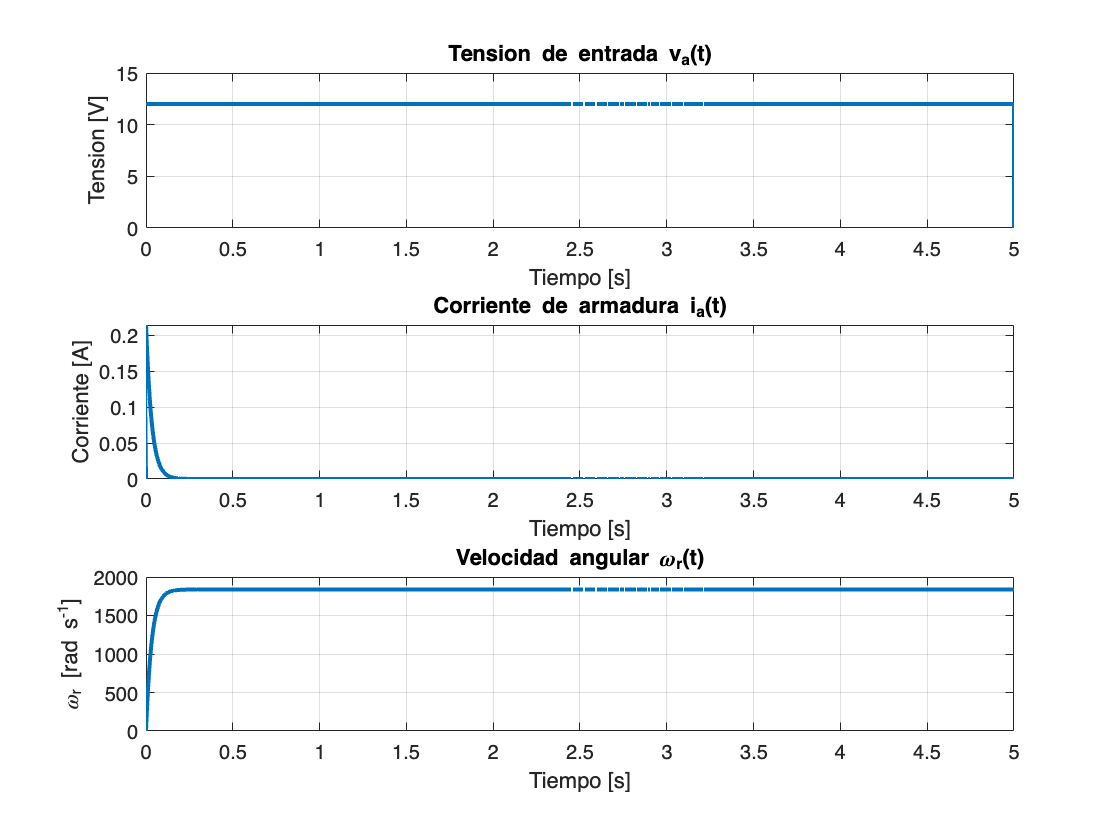
\includegraphics[width=\maxwidth{56.196688409433015em}]{figure_1.png}
\end{center}

\begin{par}
\begin{flushleft}
El problema pide mostrar simulaciones de $5\;\textrm{seg}$ que permitan observar la corriente $i_a$ en todo momento y establecer su valor pico para poder dimensionar dispositivos electrónicos. El gráfico de la corriente puede verse en la figura anterior. A continuación se muestra el pico de esa corriente.
\end{flushleft}
\end{par}

\begin{matlabcode}
disp('El pico de corriente es de:')
\end{matlabcode}
\begin{matlaboutput}
El pico de corriente es de:
\end{matlaboutput}
\begin{matlabcode}
iMax = max(Ial)
\end{matlabcode}
\begin{matlaboutput}
iMax = 0.2146
\end{matlaboutput}

\begin{par}
\begin{flushleft}
Ahora, para obtener el torque máximo que puede soportar el motor cuando se le aplica una entrada de tensión de $12V$, se puede utilizar la ecuación que modela el torque. Es decir:
\end{flushleft}
\end{par}

\begin{par}
$$T=K_i i_a$$
\end{par}

\begin{par}
\begin{flushleft}
Siendo que se conoce el máximo de la corriente para la entrada definida, simplemente restaría evaluar la expresión anterior para las condiciones dadas:
\end{flushleft}
\end{par}

\begin{matlabcode}
Tmax = Ki*iMax
\end{matlabcode}
\begin{matlaboutput}
Tmax = 0.0014
\end{matlaboutput}

\begin{par}
\begin{flushleft}
Finalmente, el torque máximo que puede soportar el motor para estas condiciones de funcionamiento es de $1\ldotp 4\;{10}^{-3} \;\textrm{Nm}$.
\end{flushleft}
\end{par}


\begin{par}
\begin{flushleft}
Ahora, para poder implementar el modelado de un sistema MIMO, es decir, múltiples entradas y múltiples salidas, se transforma el sistema de ecuaciones diferenciales al dominio de Laplace, para poder así despejar lo necesario. Se utilizará el paquete simbólico para esta tarea.
\end{flushleft}
\end{par}

\begin{par}
$${\textrm{sI}}_a \left(s\right)=-\frac{R_A \;}{L_{\textrm{AA}} }I_a \left(s\right)-\frac{K_m \;}{L_{\textrm{AA}} }\Omega {\;}_r \left(s\right)+\frac{1\;}{L_{\textrm{AA}} }V_a \left(s\right)$$
\end{par}

\begin{par}
$$s\Omega {\;}_r \left(s\right)=\frac{K_i \;}{J}I_a \left(s\right)-\frac{B_m \;}{J}\Omega {\;}_r \left(s\right)-\frac{1\;}{J}T_L \left(s\right)$$
\end{par}

\begin{par}
$$s\Theta {\;}_t =\Omega {\;}_r \left(s\right)$$
\end{par}

\begin{matlabcode}
syms s I_a R_A L_AA K_m Omega_r V_a K_i J B_m Theta_t real;
eq1 = s*I_a == -(R_A/L_AA)*I_a-(K_m/L_AA)*Omega_r+(1/L_AA)*V_a
\end{matlabcode}
\begin{matlabsymbolicoutput}
eq1 = 

\hskip1em $\displaystyle I_a \,s=\frac{V_a }{L_{\textrm{AA}} }-\frac{K_m \,\Omega_r }{L_{\textrm{AA}} }-\frac{I_a \,R_A }{L_{\textrm{AA}} }$
\end{matlabsymbolicoutput}
\begin{matlabcode}
eq2 = s*Omega_r == (K_i/J)*I_a-(B_m/J)*Omega_r
\end{matlabcode}
\begin{matlabsymbolicoutput}
eq2 = 

\hskip1em $\displaystyle \Omega_r \,s=\frac{I_a \,K_i }{J}-\frac{B_m \,\Omega_r }{J}$
\end{matlabsymbolicoutput}

\begin{par}
\begin{flushleft}
Se obtienen las funciones de transferencia que relacionan la velocidad angular y la corriente con la tensión de entrada, para ello se pasiva la entrada de $T_L$.
\end{flushleft}
\end{par}

\begin{matlabcode}
Omega_r = solve(eq2,Omega_r)
\end{matlabcode}
\begin{matlabsymbolicoutput}
Omega\_r = 

\hskip1em $\displaystyle \frac{I_a \,K_i }{B_m +J\,s}$
\end{matlabsymbolicoutput}
\begin{matlabcode}
eq1 = eval(eq1)
\end{matlabcode}
\begin{matlabsymbolicoutput}
eq1 = 

\hskip1em $\displaystyle I_a \,s=\frac{V_a }{L_{\textrm{AA}} }-\frac{I_a \,R_A }{L_{\textrm{AA}} }-\frac{I_a \,K_i \,K_m }{L_{\textrm{AA}} \,{\left(B_m +J\,s\right)}}$
\end{matlabsymbolicoutput}
\begin{matlabcode}
Ia_Va = collect(simplify(solve(eq1,I_a)/V_a))
\end{matlabcode}
\begin{matlabsymbolicoutput}
Ia\_Va = 

\hskip1em $\displaystyle \frac{J\,s+B_m }{{\left(J\,L_{\textrm{AA}} \right)}\,s^2 +{\left(B_m \,L_{\textrm{AA}} +J\,R_A \right)}\,s+B_m \,R_A +K_i \,K_m }$
\end{matlabsymbolicoutput}
\begin{matlabcode}
syms I_a Omega_r real;
eq1 = s*I_a == -(R_A/L_AA)*I_a-(K_m/L_AA)*Omega_r+(1/L_AA)*V_a;
eq2 = s*Omega_r == (K_i/J)*I_a-(B_m/J)*Omega_r;
I_a = solve(eq2,I_a)
\end{matlabcode}
\begin{matlabsymbolicoutput}
I\_a = 

\hskip1em $\displaystyle \frac{B_m \,\Omega_r +J\,\Omega_r \,s}{K_i }$
\end{matlabsymbolicoutput}
\begin{matlabcode}
eq1 = collect(eval(eq1))
\end{matlabcode}
\begin{matlabsymbolicoutput}
eq1 = 

\hskip1em $\displaystyle \frac{J\,\Omega_r }{K_i }\,s^2 +\frac{B_m \,\Omega_r }{K_i }\,s={\left(-\frac{J\,\Omega_r \,R_A }{K_i \,L_{\textrm{AA}} }\right)}\,s+\frac{V_a }{L_{\textrm{AA}} }-\frac{K_m \,\Omega_r }{L_{\textrm{AA}} }-\frac{B_m \,\Omega_r \,R_A }{K_i \,L_{\textrm{AA}} }$
\end{matlabsymbolicoutput}
\begin{matlabcode}
Omegar_Va = collect(simplify(solve(eq1,Omega_r)/V_a))
\end{matlabcode}
\begin{matlabsymbolicoutput}
Omegar\_Va = 

\hskip1em $\displaystyle \frac{K_i }{{\left(J\,L_{\textrm{AA}} \right)}\,s^2 +{\left(B_m \,L_{\textrm{AA}} +J\,R_A \right)}\,s+B_m \,R_A +K_i \,K_m }$
\end{matlabsymbolicoutput}

\begin{par}
\begin{flushleft}
Siendo que la posición angular es definida como la integral de la velocidad angular, para obtener la función de transferencia de la misma basta simplemente con la aplicación de un integrador a la última función de transferencia obtenida. De esta forma se obtiene:
\end{flushleft}
\end{par}

\begin{matlabcode}
Thetar_Va = collect(simplify(Omegar_Va/s))
\end{matlabcode}
\begin{matlabsymbolicoutput}
Thetar\_Va = 

\hskip1em $\displaystyle \frac{K_i }{{\left(J\,L_{\textrm{AA}} \right)}\,s^3 +{\left(B_m \,L_{\textrm{AA}} +J\,R_A \right)}\,s^2 +{\left(B_m \,R_A +K_i \,K_m \right)}\,s}$
\end{matlabsymbolicoutput}

\begin{par}
\begin{flushleft}
Ahora, para las funciones de transferencia que involucran al torque de carga como variable de entrada:
\end{flushleft}
\end{par}

\begin{matlabcode}
syms s I_a R_A L_AA K_m Omega_r K_i J B_m T_L Theta_t real;
eq1 = s*I_a == -(R_A/L_AA)*I_a-(K_m/L_AA)*Omega_r
\end{matlabcode}
\begin{matlabsymbolicoutput}
eq1 = 

\hskip1em $\displaystyle I_a \,s=-\frac{K_m \,\Omega_r }{L_{\textrm{AA}} }-\frac{I_a \,R_A }{L_{\textrm{AA}} }$
\end{matlabsymbolicoutput}
\begin{matlabcode}
eq2 = s*Omega_r == (K_i/J)*I_a-(B_m/J)*Omega_r-(1/J)*T_L
\end{matlabcode}
\begin{matlabsymbolicoutput}
eq2 = 

\hskip1em $\displaystyle \Omega_r \,s=\frac{I_a \,K_i }{J}-\frac{B_m \,\Omega_r }{J}-\frac{T_L }{J}$
\end{matlabsymbolicoutput}
\begin{matlabcode}
Omega_r = solve(eq1,Omega_r);
eq2 = eval(eq2);
I_a = solve(eq2,I_a)
\end{matlabcode}
\begin{matlabsymbolicoutput}
I\_a = 

\hskip1em $\displaystyle \frac{T_L }{J\,{\left(\frac{K_i }{J}+\frac{s\,{\left(R_A +L_{\textrm{AA}} \,s\right)}}{K_m }+\frac{B_m \,{\left(R_A +L_{\textrm{AA}} \,s\right)}}{J\,K_m }\right)}}$
\end{matlabsymbolicoutput}
\begin{matlabcode}
Ia_TL = collect(simplify(I_a/T_L))
\end{matlabcode}
\begin{matlabsymbolicoutput}
Ia\_TL = 

\hskip1em $\displaystyle \frac{K_m }{{\left(J\,L_{\textrm{AA}} \right)}\,s^2 +{\left(B_m \,L_{\textrm{AA}} +J\,R_A \right)}\,s+B_m \,R_A +K_i \,K_m }$
\end{matlabsymbolicoutput}
\begin{matlabcode}
syms I_a Omega_r real;
eq1 = s*I_a == -(R_A/L_AA)*I_a-(K_m/L_AA)*Omega_r;
eq2 = s*Omega_r == (K_i/J)*I_a-(B_m/J)*Omega_r-(1/J)*T_L;
I_a = solve(eq1,I_a);
eq2 = eval(eq2);
Omega_r = solve(eq2,Omega_r);
Omegar_TL = collect(simplify(Omega_r/T_L))
\end{matlabcode}
\begin{matlabsymbolicoutput}
Omegar\_TL = 

\hskip1em $\displaystyle \frac{{\left(-L_{\textrm{AA}} \right)}\,s-R_A }{{\left(J\,L_{\textrm{AA}} \right)}\,s^2 +{\left(B_m \,L_{\textrm{AA}} +J\,R_A \right)}\,s+B_m \,R_A +K_i \,K_m }$
\end{matlabsymbolicoutput}
\begin{matlabcode}
Thetar_TL = collect(simplify(Omegar_TL/s))
\end{matlabcode}
\begin{matlabsymbolicoutput}
Thetar\_TL = 

\hskip1em $\displaystyle \frac{{\left(-L_{\textrm{AA}} \right)}\,s-R_A }{{\left(J\,L_{\textrm{AA}} \right)}\,s^3 +{\left(B_m \,L_{\textrm{AA}} +J\,R_A \right)}\,s^2 +{\left(B_m \,R_A +K_i \,K_m \right)}\,s}$
\end{matlabsymbolicoutput}

\begin{par}
\begin{flushleft}
Anteriormente se obtuvieron las diferentes funciones de transferencia del sistema. Con ello, es posible plantear una matriz para un sistema MIMO, en donde cada posición de la misma relacione una entrada con una salida del sistema. Las columnas representan las entradas y las filas las salidas. Se puede resumir entonces el sistema en:
\end{flushleft}
\end{par}

\begin{matlabcode}
[Ia_Va Ia_TL; Omegar_Va Omegar_TL; Thetar_Va Thetar_TL]
\end{matlabcode}
\begin{matlabsymbolicoutput}
ans = 

\hskip1em $\displaystyle \begin{array}{l}
\left(\begin{array}{cc}
\frac{J\,s+B_m }{\sigma_1 } & \frac{K_m }{\sigma_1 }\\
\frac{K_i }{\sigma_1 } & \frac{{\left(-L_{\textrm{AA}} \right)}\,s-R_A }{\sigma_1 }\\
\frac{K_i }{\sigma_2 } & \frac{{\left(-L_{\textrm{AA}} \right)}\,s-R_A }{\sigma_2 }
\end{array}\right)\\
\mathrm{}\\
\textrm{where}\\
\mathrm{}\\
\;\;\sigma_1 ={\left(J\,L_{\textrm{AA}} \right)}\,s^2 +{\left(B_m \,L_{\textrm{AA}} +J\,R_A \right)}\,s+B_m \,R_A +K_i \,K_m \\
\mathrm{}\\
\;\;\sigma_2 ={\left(J\,L_{\textrm{AA}} \right)}\,s^3 +{\left(B_m \,L_{\textrm{AA}} +J\,R_A \right)}\,s^2 +{\left(B_m \,R_A +K_i \,K_m \right)}\,s
\end{array}$
\end{matlabsymbolicoutput}

\begin{par}
\begin{flushleft}
Es importante notar que las ecuaciones carácterísticas son exactamente iguales para las primeras 4 funciones de transferencia, lo que corrobora el modelado. Y luego, las funciones que relacionan la salida de $\Theta {\;}_t$ tienen la misma ecuación característica también, que resulta del producto entre las primeras ecuaciones carácterísticas por la variable de Laplace $s$.
\end{flushleft}
\end{par}


\begin{par}
\begin{flushleft}
A continuación, se graficarán las mediciones presentes en el archivo de Excel:
\end{flushleft}
\end{par}

\begin{matlabcode}
filename = 'GitHub/TPsControl2/Actividad 1/curvasMotor.xlsx';
sheet = 1;
t = xlsread(filename,sheet,'A1:A31054');
w = xlsread(filename,sheet,'B1:B31054');
i = xlsread(filename,sheet,'C1:C31054');
v = xlsread(filename,sheet,'D1:D31054');
T = xlsread(filename,sheet,'E1:E31054');

subplot(4,1,1);
plot(t,w,'LineWidth',2);
ylabel('\omega_r [rad s^{-1}');
xlabel('Tiempo [s]');
subplot(4,1,2);
plot(t,i,'LineWidth',2);
ylabel('i_a [A]');
xlabel('Tiempo [s]');
subplot(4,1,3);
plot(t,v,'LineWidth',2);
ylabel('V_a [V]');
xlabel('Tiempo [s]');
subplot(4,1,4);
plot(t,T,'LineWidth',2);
ylabel('T_L [Nm]');
xlabel('Tiempo [s]');
\end{matlabcode}
\begin{center}
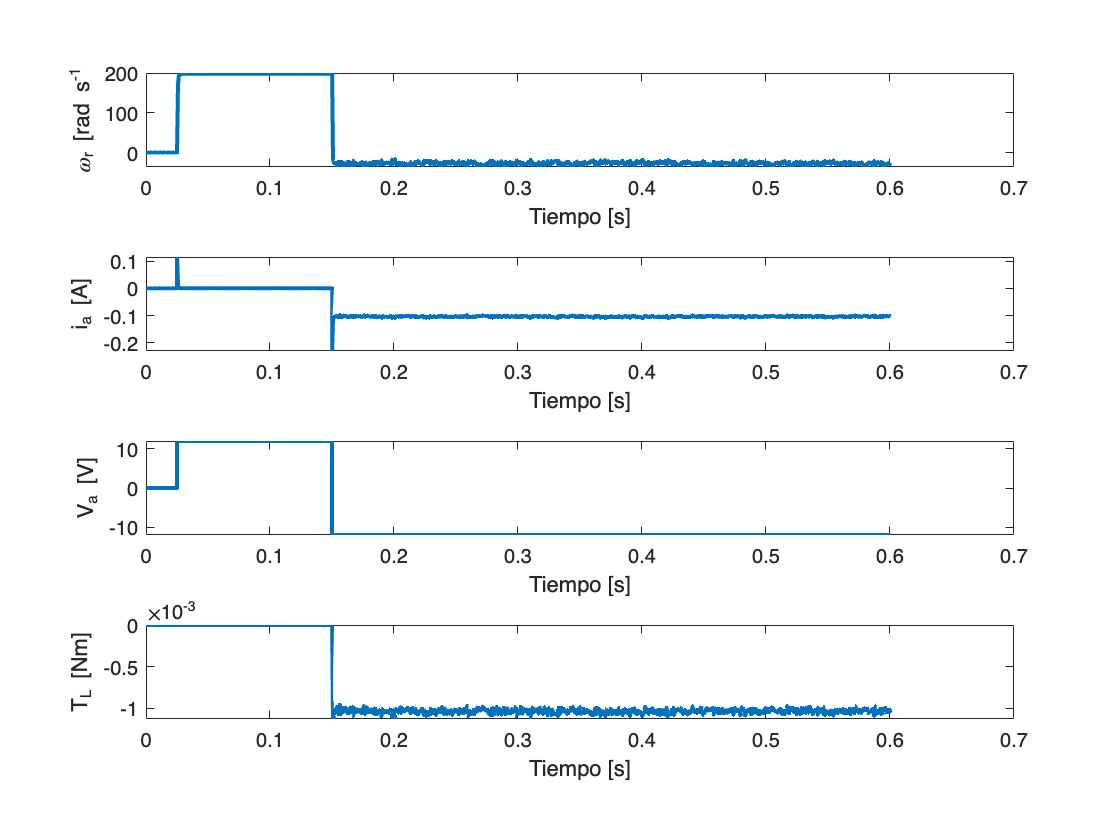
\includegraphics[width=\maxwidth{56.196688409433015em}]{figure_2.png}
\end{center}


\begin{par}
\begin{flushleft}
Para reconocer la función de transferencia junto con sus constantes escalares, se utiliza el método de Chen. Para ello, se define $t_1 =1\ldotp 9\;{10}^{-6} \;\textrm{seg}$. Se tienen así entonces:
\end{flushleft}
\end{par}

\begin{itemize}
\setlength{\itemsep}{-1ex}
   \item{\begin{flushleft} $\displaystyle y\left(t_1 \right)=0\ldotp 13231206$ \end{flushleft}}
   \item{\begin{flushleft} $\displaystyle y\left(2t_1 \right)=0\ldotp 51227978$ \end{flushleft}}
   \item{\begin{flushleft} $\displaystyle y\left(3t_1 \right)=1\ldotp 0610847$ \end{flushleft}}
   \item{\begin{flushleft} $\displaystyle K=198$ \end{flushleft}}
\end{itemize}

\begin{matlabcode}
t1 = 1.9e-6;
y1 = 0.13231206;
y2 = 0.51227978;
y3 = 1.0610847;
K = 198;

k1 = (y1/K)-1
\end{matlabcode}
\begin{matlaboutput}
k1 = -0.9993
\end{matlaboutput}
\begin{matlabcode}
k2 = (y2/K)-1
\end{matlabcode}
\begin{matlaboutput}
k2 = -0.9974
\end{matlaboutput}
\begin{matlabcode}
k3 = (y3/K)-1
\end{matlabcode}
\begin{matlaboutput}
k3 = -0.9946
\end{matlaboutput}
\begin{matlabcode}
b = 4*k1^3*k3-3*k1^2*k2^2-4*k2^3+k3^2+6*k1*k2*k3
\end{matlabcode}
\begin{matlaboutput}
b = 1.4864e-07
\end{matlaboutput}
\begin{matlabcode}
alpha1 = (k1*k2+k3-sqrt(b))/(2*(k1^2+k2))
\end{matlabcode}
\begin{matlaboutput}
alpha1 = 0.6872
\end{matlaboutput}
\begin{matlabcode}
alpha2 = (k1*k2+k3+sqrt(b))/(2*(k1^2+k2))
\end{matlabcode}
\begin{matlaboutput}
alpha2 = 0.9953
\end{matlaboutput}
\begin{matlabcode}
beta = (2*k1^3+3*k1*k2+k3-sqrt(b))/sqrt(b)
\end{matlabcode}
\begin{matlaboutput}
beta = -2.0260
\end{matlaboutput}
\begin{matlabcode}
T1 = -t1/(log(alpha1))
\end{matlabcode}
\begin{matlaboutput}
T1 = 5.0649e-06
\end{matlaboutput}
\begin{matlabcode}
T2 = -t1/(log(alpha2))
\end{matlabcode}
\begin{matlaboutput}
T2 = 4.0530e-04
\end{matlaboutput}
\begin{matlabcode}
T3 = beta*(T1-T2)+T1
\end{matlabcode}
\begin{matlaboutput}
T3 = 8.1595e-04
\end{matlaboutput}
\begin{matlabcode}
s = tf('s');
G = minreal(((K/12))/((T1*s+1)*(T2*s+1)))
\end{matlabcode}
\begin{matlaboutput}
G =
 
           8.038e09
  ---------------------------
  s^2 + 1.999e05 s + 4.871e08
 
Continuous-time transfer function.
Model Properties
\end{matlaboutput}
\begin{matlabcode}
[u, t] = step(12*G); 
plot(t,u,'LineWidth',3);
title('Respuesta ante escalón de 12V');
xlabel('Tiempo [s]');
ylabel('\omega_r [rad s^{-1}]');
grid;
\end{matlabcode}
\begin{center}
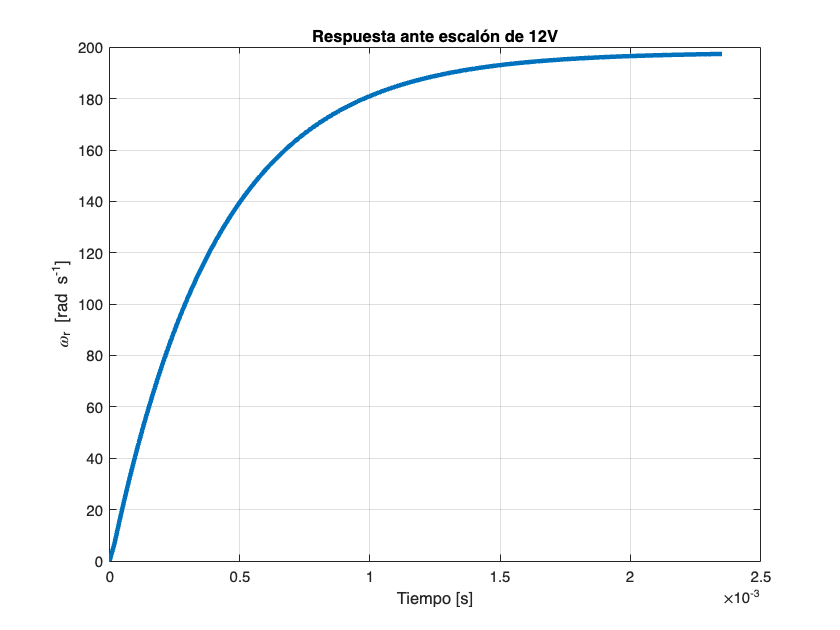
\includegraphics[width=\maxwidth{56.196688409433015em}]{figure_3.png}
\end{center}

\begin{par}
\begin{flushleft}
Se puede comprobar mediante la gráfica, que la aproximación a la función de transferencia $G\left(s\right)=\frac{\Omega {\;}_r \left(s\right)\;}{V_a \left(s\right)}$ es correcta. Ahora, con la definición de la misma se obtienen los parámetros intervinientes. Para que la función de transferencia tenga la forma que tiene la que devuelve Matlab, es necesario expresarla de otra manera, por ello se expresa la ecuación característica como:
\end{flushleft}
\end{par}

\begin{par}
\begin{flushleft}
$D\left(s\right)=s^2 +\frac{R_A }{L_{\textrm{AA}} }s+\frac{K_i K_m \;}{L_{\textrm{AA}} J}$.
\end{flushleft}
\end{par}

\begin{par}
\begin{flushleft}
Como se tienen más incógnitas que ecuaciones, se debe suponer un valor de $L_{\textrm{AA}}$, se utiliza el de la consigna: $L_{\textrm{AA}} =366\mu \;\textrm{Hy}$, lo mismo sucede con el valor de $J=5\;{10}^{-9} \textrm{Kg}\;m^2$. Con eso:
\end{flushleft}
\end{par}

\begin{itemize}
\setlength{\itemsep}{-1ex}
   \item{\begin{flushleft} $\displaystyle R_A =1\ldotp 999\;{10}^5 *366\;{10}^{-6} =73\ldotp 17\;\Omega \;$ \end{flushleft}}
\end{itemize}

\begin{par}
\begin{flushleft}
Luego, generalmente en los motores de corriente continua, las constantes de fuerza electromotriz y de torque poseen valores numéricos muy aproximados (obviando las unidades). Con esto en mente, es posible aproximar $K=K_i =K_m \Rightarrow K_i K_m =K^2$, es decir:
\end{flushleft}
\end{par}

\begin{itemize}
\setlength{\itemsep}{-1ex}
   \item{\begin{flushleft} $\displaystyle K^2 =4\ldotp 871\;{10}^8 \;\;366\;{10}^{-6} \;\;5\;{10}^{-9} =8\ldotp 91\;{10}^{-4} \Rightarrow K=29\ldotp 8\;{10}^{-3}$ \end{flushleft}}
\end{itemize}

\begin{par}
\begin{flushleft}
Con los valores de las constantes determinados, se debe obtener de forma numérica la función de transferencia de la velocidad angular relacionada al torque. 
\end{flushleft}
\end{par}

\begin{par}
$$\frac{\Omega {\;}_r \left(s\right)}{T_L \left(s\right)}=\frac{-366\;{10}^{-6} s-73\ldotp 17}{1\ldotp 83\;{10}^{-12} s^3 +3\ldotp 66\;{10}^{-7} s^2 +8\ldotp 91\;{10}^{-4} s}$$
\end{par}

\begin{matlabcode}
OmegaT = tf([-366e-6 -73.17], [1.82e-12 3.66e-7 8.91e-4 0])
\end{matlabcode}
\begin{matlaboutput}
OmegaT =
 
            -0.000366 s - 73.17
  ----------------------------------------
  1.82e-12 s^3 + 3.66e-07 s^2 + 0.000891 s
 
Continuous-time transfer function.
Model Properties
\end{matlaboutput}


\begin{par}
\begin{flushleft}
Ahora se definen las dos entradas del sistema tal cual son vistas en el documento que almacena los datos de medición, de forma de corroborar que las funciones de transferencia obtenidas sean correctas:
\end{flushleft}
\end{par}

\begin{matlabcode}
T = 0.6;
t = 0:0.0001:T;
t1 = t(t>=0 & t<0.025);
t2 = t(t>=0.025 & t<0.15);
t3 = t(t>=0.15);

v1 = 0*t1;
v2 = 0*t2+12;
v3 = 0*t3-12;
v = [v1 v2 v3];

tl1 = 0*t1;
tl2 = 0*t2;
tl3 = 0*t3-0.00103;
tl =[tl1 tl2 tl3];

Ki = 29.8e-3;
Km = Ki;
Laa = 366e-6;
J = 5e-9;
Ra = 73.17;
Bm = 0;

A = [-Ra/Laa -Km/Laa; Ki/J -Bm/J];
B = [1/Laa; -1/J];
C = [0 1];
D = [1 1];

sys = ss(A,B,C,D)
\end{matlabcode}
\begin{matlaboutput}
Error using ss
The "B" and "D" matrices must have the same number of columns.
\end{matlaboutput}
\begin{matlabcode}

\end{matlabcode}

\end{document}
